\section{Simulation Study}
\label{c2:sec:simulation_study}
In Section~\ref{c2:subsec:demo_prias_pers_schedule} we demonstrated that the personalized schedules, schedule future biopsies according to the historical data of each patient. However, we could not perform a full-scale comparison between personalized and PRIAS schedules, because the true time of GR was not known for the PRIAS patients. To this end, we conducted a simulation study comparing personalized schedules with PRIAS and annual schedule, whose details are presented next.

\subsection{Simulation Setup}
\label{c2:subsec:simulation_setup}
The population of AS patients in this simulation study is assumed to have the same entrance criteria as that of PRIAS. The PSA and hazard of GR for these patients follow a joint model of the form postulated in Section~\ref{c2:subsec:jm_fit_prias}, with the only change that $\log_2 \mbox{PSA}$ levels are used as the outcome. The population joint model parameters are equal to the posterior mean of parameters estimated from the corresponding joint model fitted to the PRIAS dataset. We intend to test the efficacy of different schedules for a population which has patients with both faster as well as slowly-progressing PCa. This rate of progression is not only manifested via PSA profiles but also via the baseline hazard. We assume that there are three equal sized subgroups $G_1$, $G_2$ and $G_3$ of patients in the population, each with a baseline hazard from a Weibull distribution, with the following shape and scale parameters $(k, \lambda$): $(1.5, 4)$, $(3, 5)$ and $(4.5, 6)$ for $G_1, G_2$ and $G_3$, respectively. The effect of these parameters is that the mean GR time is lowest in $G_1$ (fast PCa progression) and highest in $G_3$ (slow PCa progression).

From this population, we have sampled 500 datasets with 1000 patients each. We generate a true GR time for each of the patients, and then sample a set of PSA measurements at the same time points as given in PRIAS protocol (quarterly for the first two years of AS, semiannually thereafter). We then split the dataset into a training (750 patients) and a test (250 patients) part, and generate a random and non-informative censoring time for the training patients. We next fit a joint model of the specification given in (\ref{c2:eq:long_model_prias}) and (\ref{c2:eq:hazard_prias}) to each of the 500 training datasets and obtain MCMC samples from the 500 sets of the posterior distribution of the parameters. Using these fitted joint models, we obtain the posterior predictive distribution of time of GR for each of the $500 \times 250$ test patients. This distribution is further used to create personalized biopsy schedules for the test patients. For every test patient we conduct hypothetical biopsies using the following six types of schedules (abbreviated names in parenthesis): personalized schedules based on expected time of GR (Exp.~GR~Time) and median time of GR (Med.~GR~Time), personalized schedules based on dynamic risk of GR (Dyn.~Risk~GR), a hybrid approach between median time of GR and dynamic risk of GR (Hybrid), PRIAS schedule and the annual schedule. The biopsies are conducted as per the algorithm in Figure~\ref{c2:fig:1}. 

To compare the aforementioned schedules we require estimates of the various measures of efficacy described in Section~\ref{c2:sec:choosing_schedule}. To this end, for schedule $S$, we compute pooled estimates of mean offset $E(O^S_j)$ and variance of offset $\mbox{var}(O^S_j)$, as below (estimates for $N^S_j$ are similar):
\begin{align*}
\widehat{E(O^S_j)} &= \frac{\sum_{k=1}^{500} n_k \widehat{E(O^S_k)}}{\sum_{k=1}^{500} n_k}, \\
\widehat{\mbox{var}(O^S_j)} &= \frac{\sum_{k=1}^{500} (n_k - 1) \widehat{\mbox{var}(O^S_k)}}{\sum_{k=1}^{500} (n_k-1)}, 
\end{align*}
where $n_k$ denotes the number of test patients, $\widehat{E(O^S_k)} = {\sum_{l=1}^{n_k}O^S_{kl}}/{n_k}$ is the estimated mean and $\widehat{\mbox{var}(O^S_k)} = {\sum_{l=1}^{n_k}\big\{O^S_{kl} - \widehat{E(O^S_k)}\big\}^2}/(n_k-1)$ is the estimated variance of the offset for the $k$-th simulation. The offset for the $l$-th test patient of the $k$-th dataset is denoted by $O^S_{kl}$.

\subsection{Results}
The pooled estimates of the aforementioned measures are summarized in Table~\ref{c2:table:sim_study_pooled_estimates_all} and Table~\ref{c2:table:sim_study_pooled_estimates_subgroup}. In addition, estimated values of $E(O^S_j)$ are plotted against $E(N^S_j)$ in Figure~\ref{c2:fig:3}. The figure shows that across the schedules, there is an inverse relationship between number $E(O^S_j)$ and $E(N^S_j)$. For example, the annual schedule conducts, on average, 5.2 biopsies to detect GR, which is the highest among all schedules. However, it has the least average offset of 6 months as well. On the other hand, the schedule based on the expected time of GR conducts only 1.9 biopsies on average to detect GR, the least among all schedules, but it also has the highest average offset of 15 months (similar for the median time of GR). Since the annual schedule attempts to contain the offset within a year it has the least $\mbox{SD}(O^S_j) = \sqrt{\mbox{var}(O^S_j)}$. However to achieve this, it conducts a wide range of number of biopsies from patient to patient, i.e., highest $\mbox{SD}(N^S_j) = \sqrt{\mbox{var}(N^S_j)}$. In this regard, schedules based on expected and median time of GR perform the opposite of the annual schedule.

\begin{figure}
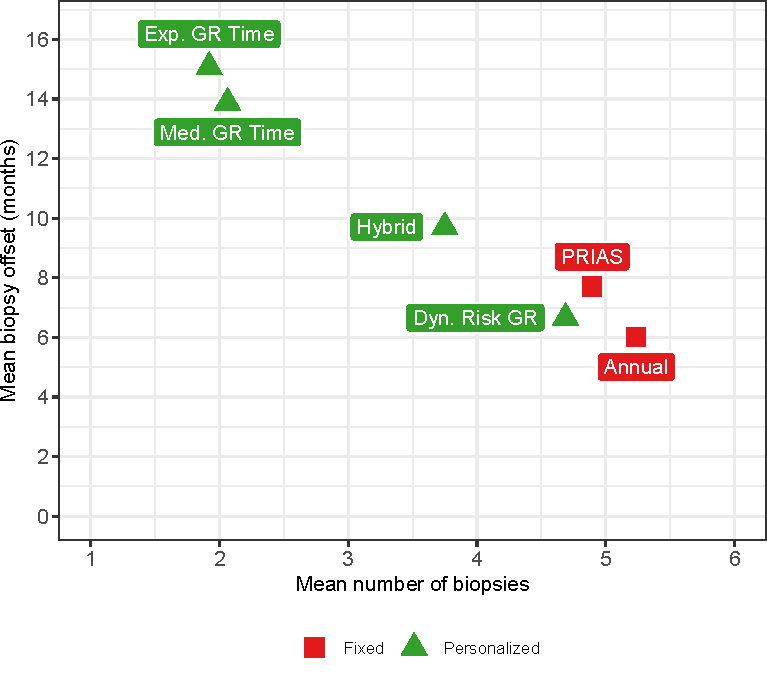
\includegraphics{contents/c2/images/c2_fig3.pdf}
\caption{\textbf{Estimated mean number of biopsies and offset (in months)}. Biopsies are conducted until Gleason reclassification (GR) is detected. Offset is the difference in time at which GR is detected and the true time of GR. Results are based on the simulated (500 datasets) test patients. \textbf{Types of personalized schedules}: Exp.~GR~Time (expected time of GR), Med.~GR~Time (median time of GR), Dyn.~Risk~GR (schedules based on the dynamic risk of GR), Hybrid (a hybrid approach between Med.~GR~Time and Dyn.~Risk~GR). \textbf{Annual}: yearly biopsies. \textbf{PRIAS}: biopsies as per PRIAS protocol.}
\label{c2:fig:3}
\end{figure}

%124781 = 41484 + 41423 + 41874
\begin{table}
\small
\centering
\caption{\textbf{Estimated mean and standard deviation (SD), of the number of biopsies $N^S_j$ and offset $O^S_j$}. Offset (in months) is defined as difference in time at which GR (Gleason reclassification) is detected and the true time of GR. Results are based on all simulated (500 datasets) test patients. \textbf{Types of personalized schedules}: Exp.~GR~Time (expected time of GR), Med.~GR~Time (median time of GR), Dyn.~Risk~GR (schedules based on dynamic risk of GR), Hybrid (a hybrid approach between Med.~GR~Time and Dyn.~Risk~GR). \textbf{Annual}: yearly biopsies. \textbf{PRIAS}: biopsies as per PRIAS protocol.}
\label{c2:table:sim_study_pooled_estimates_all}
\begin{tabular}{lrrrr}
\toprule
Schedule          & $E(N^S_j)$ & $E(O^S_j)$ & ${\mbox{SD}(N^S_j)}$ & ${\mbox{SD}(O^S_j)}$ \\
\midrule
Annual         & 5.24            & 6.01                & 2.53          & 3.46              \\
PRIAS          & 4.90            & 7.71                & 2.36          & 6.31\\
Dyn.~Risk~GR       & 4.69            & 6.66                & 2.19           & 4.38              \\
Hybrid       & 3.75            & 9.70                & 1.71          & 7.25              \\
Med.~GR~Time & 2.06            & 13.88               & 1.41          & 11.80              \\
Exp.~GR~Time & 1.92            & 15.08               & 1.19          & 12.11             \\
\bottomrule
\end{tabular}
\end{table}

\begin{table}
\small
\centering
\caption{\textbf{Subgroup Estimated mean and standard deviation (SD), of the number of biopsies $N^S_j$ and offset $O^S_j$}. Offset (in months) is defined as difference in time at which GR (Gleason reclassification) is detected and the true time of GR. Results based on simulated (500 datasets) test patients, with \textbf{Subgroup $G_1$} and \textbf{Subgroup $G_3$} having the fastest, and slowest progressing cancer patients, respectively. \textbf{Types of personalized schedules}: Exp.~GR~Time (expected time of GR), Med.~GR~Time (median time of GR), Dyn.~Risk~GR (schedules based on dynamic risk of GR), Hybrid (a hybrid approach between Med.~GR~Time and Dyn.~Risk~GR). \textbf{Annual}: yearly biopsies. \textbf{PRIAS}: biopsies as per PRIAS protocol.}
\label{c2:table:sim_study_pooled_estimates_subgroup}
\begin{tabular}{lrrrr}
\toprule
\multicolumn{5}{c}{b) Hypothetical subgroup $G_1$}\\
\midrule
Schedule        & $E(N^S_j)$ & $E(O^S_j)$ & ${\mbox{SD}(N^S_j)}$ & ${\mbox{SD}(O^S_j)}$ \\
\midrule
Annual         & 4.32            & 6.02                & 3.13          & 3.44              \\
PRIAS          & 4.07            & 7.44                & 2.88          & 6.11    \\
Dyn.~Risk~GR       & 3.85            & 6.75                & 2.69          & 4.44              \\
Hybrid       & 3.25            & 10.25               & 2.16          & 8.07              \\
Med.~GR~Time & 1.84            & 20.66               & 1.76          & 14.62             \\
Exp.~GR~Time & 1.72            & 21.65               & 1.47          & 14.75             \\
\midrule     
\multicolumn{5}{c}{c) Hypothetical subgroup $G_2$}\\
\midrule
Schedule        & $E(N^S_j)$ & $E(O^S_j)$ & ${\mbox{SD}(N^S_j)}$ & ${\mbox{SD}(O^S_j)}$ \\
\midrule
Annual         & 5.18            & 5.98                & 2.13          & 3.47              \\
PRIAS          & 4.85            & 7.70                & 2.00          & 6.29        \\
Dyn.~Risk~GR       & 4.63            & 6.66                & 1.82          & 4.37              \\
Hybrid       & 3.68            & 10.32                & 1.37          & 7.45              \\
Med.~GR~Time & 1.89             & 12.33               & 1.16          & 9.44              \\
Exp.~GR~Time & 1.77            & 13.54               & 0.98          & 9.83              \\
\midrule    
\multicolumn{5}{c}{d) Hypothetical subgroup $G_3$}\\
\midrule
Schedule        & $E(N^S_j)$ & $E(O^S_j)$ & ${\mbox{SD}(N^S_j)}$ & ${\mbox{SD}(O^S_j)}$ \\
\midrule
Annual         & 6.20             & 6.02                & 1.76          & 3.46              \\
PRIAS          & 5.76             & 7.98                & 1.71         & 6.51        \\
Dyn.~Risk~GR       & 5.58            & 6.58                & 1.56          & 4.33              \\
Hybrid       & 4.32            & 8.55                & 1.26          & 5.91              \\
Med.~GR~Time & 2.45            & 8.70                & 1.15          & 6.32              \\
Exp.~GR~Time & 2.27            & 10.09               & 0.99          & 7.47              \\
\bottomrule    
\end{tabular}
\end{table}

The PRIAS schedule conducts only 0.3 biopsies less than the annual schedule, but with a higher $\mbox{SD}(O^S_j)$, early detection is not always guaranteed. In comparison, the dynamic risk of GR based schedule performs slightly better than the PRIAS schedule in all four criteria. The hybrid approach combines the benefits of methods with low $E(N^S_j)$ and $\mbox{SD}(N^S_j)$, and methods with low $E(O^S_j)$ and $\mbox{SD}(O^S_j)$. It conducts 1.5 biopsies less than the annual schedule on average, and with a $E(O^S_j)$ of 9.7 months, it detects GR within a year since its occurrence. Moreover, it has both $\mbox{SD}(N^S_j)$ and $\mbox{SD}(O^S_j)$ comparable to PRIAS.

The performance of each schedule differs for the three subgroups $G_1, G_2$, and $G_3$. The annual schedule remains the most consistent across subgroups in terms of the offset, but it conducts two extra biopsies for the subgroup $G_3$ (slowly-progressing PCa) than $G_1$ (faster-progressing PCa). The performance of schedule based on expected time of GR is the most consistent in terms of the number of biopsies, but it detects GR a year later on average in subgroup $G_1$ than $G_3$. For the dynamic risk of GR based schedule and the hybrid schedule, the dynamics are similar to that of the annual schedule. Unlike the latter two schedules, the PRIAS schedule not only conducts more biopsies in $G_3$ than $G_1$ but also detects GR later in $G_3$ than $G_1$.

\begin{figure}
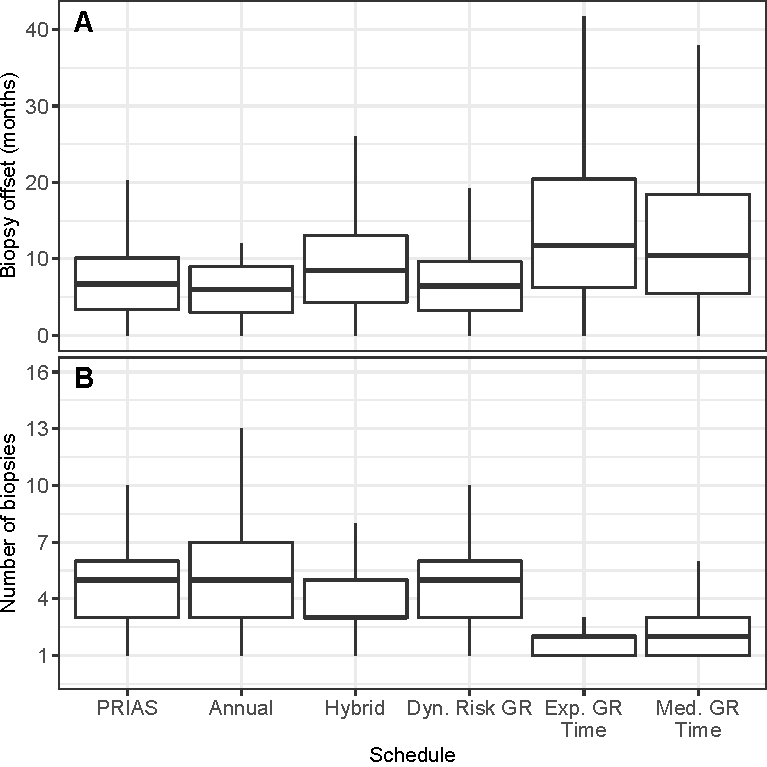
\includegraphics{contents/c2/images/c2_fig4.pdf}
\caption{Variation in the number of biopsies and biopsy offset (difference in time at which Gleason reclassification / GR is detected and the true time of GR, in months). Results are based on the simulated (500 datasets) test patients. Biopsies are conducted until Gleason reclassification (GR) is detected. \textbf{Types of personalized schedules}: Exp.~GR~Time (expected time of GR), Med.~GR~Time (median time of GR), Dyn.~Risk~GR (schedules based on the dynamic risk of GR), Hybrid (a hybrid approach between Med.~GR~Time and Dyn.~Risk~GR). \textbf{Annual}: yearly biopsies. \textbf{PRIAS}: biopsies as per PRIAS protocol.}
\label{c2:fig:4}
\end{figure}

The choice of a suitable schedule using (\ref{c2:eq:loss_func_sim_study_generic}) depends on the chosen measure for evaluation of schedules. In this regard, the schedules we compared either have high $\mbox{SD}(O^S_j)$ and low $\mbox{SD}(N^S_j)$, or vice versa (Table~\ref{c2:table:sim_study_pooled_estimates_all} and Table~\ref{c2:table:sim_study_pooled_estimates_subgroup}). Thus, applying a cutoff on $E(O^S_j)$ when $\mbox{SD}(O^S_j)$ is high may not be as fruitful (same for $N^S_j$) as applying a cutoff on $\mbox{SD}(O^S_j)$ or quantile(s) of $O^S_j$. For example, the schedule based on the dynamic risk of GR is suitable if, on average, the least number of biopsies are to be conducted to detect GR, while simultaneously making sure that at least 90\% of the patients have an average offset less than one year.